Graphs are fundamental data structures in many applications, such as computer networks, recommendation systems, and circuit design. In recent years, a number of high performance graph processing frameworks have emerged. State-of-the-art frameworks include Gunrock \cite{wang2016gunrock}, Hornet \cite{busato2018hornet}, Ligra \cite{shun2013ligra}, and Galois \cite{nguyen2013lightweight}.\ignore{These frameworks have demonstrated efficient computation on billion-scale graphs.} Their emphasis lies in accelerating graph analytics tasks by providing high-performance kernels tailored to diverse datasets.

Unfortunately, loading graph data is a significant bottleneck in such frameworks. In fact, the cost of loading data can dominate the overall processing time --- especially as computational capabilities continue to improve\ignore{\cite{gabert2021pigo}}. Gabert and Çatalyürek \cite{gabert2021pigo} observe that\ignore{even on high-performance shared-memory graph systems running billion-scale graphs,} reading the graph from file systems, on such frameworks, takes multiple orders of magnitude longer than running the computational kernel. This slowdown not only causes a disconnect for end users and a loss of productivity for researchers\ignore{/developers}, but also increases the system/cloud usage charges. Fast loading of graphs is thus, crucial\ignore{for minimizing the time it takes to start processing and analyzing the graph data}.\ignore{This motivates us to work on efficient IO techniques. These not only improve response time, but also help lower system / cloud usage charges.}

In modern frameworks like Gunrock, loading graph data from ASCII-based file formats, specifically using the Coordinate (COO) format, is a major bottleneck. To load the graph as an Edgelist, these frameworks typically follow a sequential process of opening the input file, reading the entries one by one, and inserting them into an array. If the goal is to access the graph in the Compressed Sparse Row (CSR) format, which is often the case --- due to its storage efficiency and locality benefits, additional steps are required. These include computing the out-degrees of vertices from the Edgelist, performing prefix sum to determine the offsets of outgoing edges in the CSR representation, and then populating the CSR arrays with edges from the Edgelist. All these operations are carried out sequentially, contributing to the overall loading time.

%% TEXT BELOW NEEDS REPHRASING/SUMMARIZING

We now discuss how state-of-the-art frameworks, such as Gunrock, load graphs from ASCII-based file formats, where the graph is represented using the Coordinate (COO) format. To load a graph into an Edgelist, these frameworks generally open the input file as an input file stream, sequentially read the tuples/entries, and insert them into an array. If it is desirable to access the graph in the Compressed Sparse Row (CSR) format, which in most cases it is, these frameworks use the Edgelist to compute the out-degrees of vertices, perform prefix sum to determine the offsets of outgoing edges in the CSR representation, and then fill in the CSR arrays with edges from the Edgelist. All operations are performed sequentially.

Thus, while these frameworks have demonstrated efficient computation on billion-scale graphs, they persist with sequential I/O, presumably under a longstanding belief that parallel I/O is not achievable without a dedicated parallel I/O system. In the literature, graph and matrix I/O times are rarely reported and, hence, not highly optimized \cite{gabert2021pigo}. While it is the case that SATA serializes disk access \cite{tavakkol2018mqsim}, implementing only sequential I/O misses three major and common opportunities for parallelism. First, a hardware Redundant Array of Inexpensive Disks (RAID) controller can read from multiple drives over separate SATA connections in parallel \cite{patterson1988case}. Second, Non-Volatile Memory (NVM) is now widely deployed \cite{jung2020openexpress} and provides parallelism through both SSDs and the NVM express (NVMe) interface to motherboards \cite{tavakkol2018mqsim}. Third, file systems include tuned and effective caches, supporting parallel reads and writes \cite{mathur2007new}.
% They persist with sequential I/O and do not fully exploit the capabilities of modern Hard Disk Drives (HDDs), Redundant Array of Independent Disks (RAID) controllers, Non-Volatile Memory (NVM), and file system caches \cite{gabert2021pigo}.

Memory mapping is a mechanism that maps a file or part of a file into the virtual memory space, so that files on the disk can be accessed as if they were in memory \cite{lin2014mmap}. There are many advantages of using memory mapping, especially when processing large files. - Reading from and writing to a memory-mapped file do not require the data to be copied to and from a user-space buffer while standard read/write do. - Aside from any potential page faults, reading from and writing to a memory-mapped file do not incur any overhead due to context switching. - When multiple processes map the same data into memory, they can access that data simultaneously. Read-only and shared writable mappings are shared in their entirety; private writable mappings may have their not-yet-COW (copy-on-write) pages shared \cite{lin2014mmap}.

Incorporation of Memory-Mapped I/O holds promise for improving graph loading efficiency of frameworks. A number of research studies have worked on optimizing the performance of memory mapped IO. The approaches include using a lightweight userspace memory service \cite{li2019userland}, huge pages \cite{malliotakis2021hugemap}, and asynchronous techniques \cite{imamura2019poster}. A large number of works have optimized memory mapped IO for fast low-latency storage devices \cite{song2012low, song2016efficient, papagiannis2020optimizing, papagiannis2021memory, alverti2022daxvm, leis2023virtual}. Essen et al. \cite{van2015di} and Feng et al. \cite{feng2023tricache} focus on enabling programs to efficiently process out-of-core datasets through memory mapping. Lin et al. \cite{lin2014mmap} use memory mapping capability of all modern hardware to create fast and scalable graph algorithms. They are able to to process $6.6$ billion edge Yahoo web graph faster than other graph processing frameworks, such as TurboGraph and GraphChi, with reduced complexity - both in terms of simpler data structures, and fewer lines of code. They benefit from existing page replacement policies, such as LRU.

A number of external memory graph processing frameworks focus of fast loading of graphs \cite{}. However, these frameworks focus on loading graphs in various binary storage formats. However, a large number of graphs datasets are available in serialized human readable data exchange formats. Such formats are preferred ... (why). We focus on fast loading of graphs stored in plain text formats.

Gabert and Çatalyürek \cite{gabert2021pigo} close the gap through PIGO, a simple to use, small, header-only, and dependency-free C++11 library that brings I/O improvements to graph and matrix systems. PIGO supports reading from file in parallel, with details of their secondary storage (NVMe HDD). PIGO has support for COO (coordinate-addressed matrices or graphs) and CSR (compressed sparse row matrices or graphs). COO is able to read a variety of input formats (e.g., matrix market) and exposes the read data as an edge list. The edge list is stored as multiple arrays, one for the x elements and one for the y elements (e.g., src and dst in graphs.). CSR is used to represent sparse matrices and graphs. In many cases, this is the desired format for a graph or matrix in memory. When sparse graphs or matrices are delivered in COO formats, such as matrix market or edge lists, they are frequently converted to CSR.

However, when reading EL, they take two passes, first to count the number of newlines to determine how to allocate storage, second, copy over the values appropriately. They do not split the file into chunks, but split the file into parts, where each thread operates on its own part. They allocation is done using \texttt{std::vector::resize} (not \texttt{mmap}). When converting EL to CSR; they use plain OpenMP for, thus a static schedule; they atomically increment degrees, on each thread, in a global shared vector; They then do a sequential prefix sum (on the vertex range of each thread) to obtain the offsets. Their prefix sum does not start with a zero, so they adjust for this, and patch the last offset (not exactly clear to me). They then copy over the COO over, again an OpenMP for with static schedule of size $1$. Adding to the CSR is done with atomic capture instructions.

%% ---------------------------------------------------------------------------------------------------

% x Why do HP G frameworks load graphs slowly?
% x A quick glimpse of how they do it.
% x Why do the persist with sequential IO? (Modern IO is fast)
% x What are the HP IO interfaces? (MMAP)
% x Which graphs frameworks make use of mmap? (external memory frameworks)
% x What do they focus on? (binary graph formats)
% x Why is fast loading of serialized formats important? (human readable data exchange format)
% x What have Gabert et al. done in PIGO?
% - How do we improve upon it? (link to code)

%% ---------------------------------------------------------------------------------------------------




\ignore{Recent graph computation approaches have demonstrated that a single PC can perform efficiently on billion-scale graphs. While these approaches achieve scalability by optimizing I/O operations, they do not fully exploit the capabilities of modern hard drives and processors \cite{gualdron2016m}.}

\ignore{Many implementations persist with sequential I/O, and the article challenges the prevalent notion that parallel I/O is unattainable without dedicated systems. By exploring opportunities for parallelism through hardware RAID controllers, Non-Volatile Memory (NVM), and file system caches, the article introduces a pragmatic perspective on addressing I/O challenges. Gabert et al. present PIGO, a lightweight C++11 header-only library, as a solution that, without imposing the complexities of existing graph systems, significantly enhances end-to-end performance and productivity for researchers and developers working on shared-memory multi-core servers. Experimental results underscore PIGO's potential to redefine the landscape of optimized graph loading, complementing the strengths of popular graph processing frameworks \cite{gabert2021pigo}.}


\subsection{Our Contributions}

This study introduces GVEL\footnote{\url{https://github.com/puzzlef/graph-csr-openmp}}, an optimized approach for reading Edgelists from text files and converting them to Compressed Sparse Row (CSR) format. GVEL outperforms Hornet, Gunrock, and PIGO in CSR reading by $78\times$, $112\times$, and $1.8\times$, respectively. With Edgelist reading, GVEL outperforms PIGO by $2.6\times$, achieving read rate of $1.9$ billion edges/s. GVEL exhibits good strong scaling, with a $1.9\times$ improvement for Edgelist reading and a $1.7\times$ increase for CSR reading with every doubling of threads.

Our techniques may also be useful for converting COO to CSR on the fly on parallel devices. This is important since CSR is an efficient data structure, while COO is easy to update. Per-thread COOs are not needed - we can use single COO and split it unto parts for each thread to process.

Maybe search related work on combining data to a common shared data structure. Have any others done what we have done?

Focus on hot and cold access, and when multiple processes are accessing the same file, it can be a (significant?) advantage.

Measure EL, CSR, EL + CSR ...
Details of NVME, as much as possible.
Indirect comparison with Ligra, GAPbs, and Galois (PIGO).
Details of other graphs processing frameworks, and the above
- cugraph
- networkit
- igraph?
- gunrock
- hornet
- graphblast

- adjust csr partitions
- adjust csr partitions (convert csr only)
- adjust block size
- warm vs cold on graphs
- read EL, convert CSR split on graphs



Memory mapping is a mechanism that maps a file or part of a file into the virtual memory space, so that files on the disk can be accessed as if they were in memory \cite{lin2014mmap}. There are many advantages of using memory mapping, especially when processing large files. - Reading from and writing to a memory-mapped file do not require the data to be copied to and from a user-space buffer while standard read/write do. - Aside from any potential page faults, reading from and writing to a memory-mapped file do not incur any overhead due to context switching. - When multiple processes map the same data into memory, they can access that data simultaneously. Read-only and shared writable mappings are shared in their entirety; private writable mappings may have their not-yet-COW (copy-on-write) pages shared \cite{lin2014mmap}.




% - Why fast graph loading is important?
% - Extremely high cost of loading compared to computation.
% - An issue with even popular graph processing frameworks.
% - Modern IO is fast (compared to CPU performance).
% - Storage capacities increasing, bandwidth is high, CPUs as not as fast as they used to be.
% - Common graph file formats (COO, MTX).
% - Common memory storage formats (Edgelist, CSR).
% - Work presented in this paper.




%% - Use --- for a dash.
%% - Use ``camera-ready'' for quotes.
%% - Use {\itshape very} or \textit{very} for italicized text.
%% - Use \verb|acmart| or {\verb|acmart|} for mono-spaced text.
%% - Use \url{https://capitalizemytitle.com/} for URLs.
%% - Use {\bfseries Do not modify this document.} for important boldface details.
%% - Use \ref{fig:name} for referencing.

%% For a block of pre-formatted text: 
% \begin{verbatim}
%   \renewcommand{\shortauthors}{McCartney, et al.}
% \end{verbatim}

%% For a list of items:
% \begin{itemize}
% \item the ``ACM Reference Format'' text on the first page.
% \item the ``rights management'' text on the first page.
% \item the conference information in the page header(s).
% \end{itemize}

%% For a table:
% \begin{table}
%   \caption{Frequency of Special Characters}
%   \label{tab:freq}
%   \begin{tabular}{ccl}
%     \toprule
%     Non-English or Math&Frequency&Comments\\
%     \midrule
%     \O & 1 in 1,000& For Swedish names\\
%     $\pi$ & 1 in 5& Common in math\\
%     \$ & 4 in 5 & Used in business\\
%     $\Psi^2_1$ & 1 in 40,000& Unexplained usage\\
%   \bottomrule
% \end{tabular}
% \end{table}

%% For a full-width table:
% \begin{table*}
%   \caption{Some Typical Commands}
%   \label{tab:commands}
%   \begin{tabular}{ccl}
%     \toprule
%     Command &A Number & Comments\\
%     \midrule
%     \texttt{{\char'134}author} & 100& Author \\
%     \texttt{{\char'134}table}& 300 & For tables\\
%     \texttt{{\char'134}table*}& 400& For wider tables\\
%     \bottomrule
%   \end{tabular}
% \end{table*}


%% For inline math:
% \begin{math}
%   \lim_{n\rightarrow \infty}x=0
% \end{math},

%% For a numbered equation:
% \begin{equation}
%   \lim_{n\rightarrow \infty}x=0
% \end{equation}

%% For an unnumbered equation:
% \begin{displaymath}
%   \sum_{i=0}^{\infty} x + 1
% \end{displaymath}

%% For a figure:
% \begin{figure}[h]
%   \centering
%   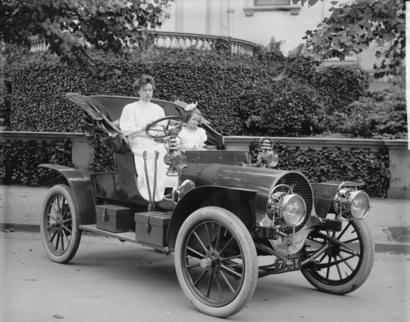
\includegraphics[width=\linewidth]{inc/sample-franklin}
%   \caption{1907 Franklin Model D roadster. Photograph by Harris \&
%     Ewing, Inc. [Public domain], via Wikimedia
%     Commons. (\url{https://goo.gl/VLCRBB}).}
%   \Description{A woman and a girl in white dresses sit in an open car.}
% \end{figure}

%% For a teaser figure.
% \begin{teaserfigure}
%   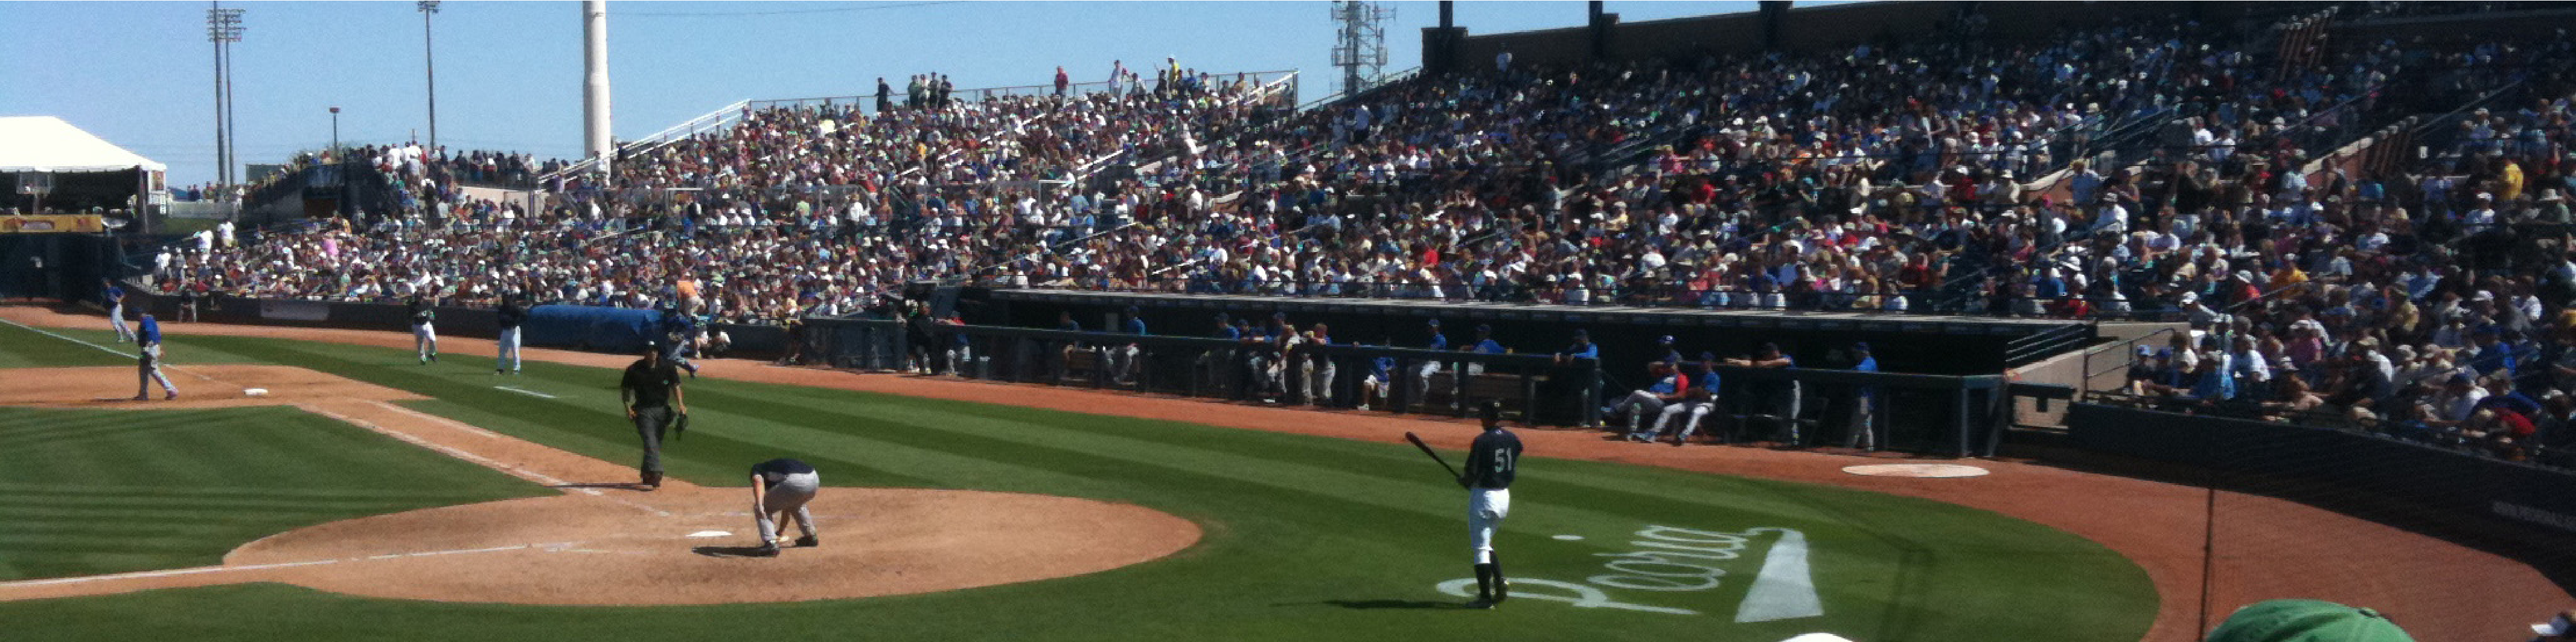
\includegraphics[width=\textwidth]{sampleteaser}
%   \caption{figure caption}
%   \Description{figure description}
% \end{teaserfigure}
